\documentclass[10pt,letterpaper,twocolumn]{article}

\usepackage[top=2.1cm,left=2.0cm,right=2.0cm,footskip=2.0cm]{geometry}
\usepackage[utf8]{inputenc}     % for Unicode
\usepackage{cite}               % citation
\usepackage[dvipdfmx]{hyperref} % links
\usepackage{caption}            % caption
\usepackage{microtype}          % improves typesetting in LaTeX
\usepackage{algpseudocode}
\usepackage{algorithm}
\usepackage{graphicx}
\usepackage{color} % ex.) \textcolor{color}{text}
\usepackage{url}

\renewcommand{\algorithmicrequire}{\textbf{Input:}}
\renewcommand{\algorithmicensure}{\textbf{Output:}}

\setcounter{topnumber}{3}
\setcounter{dbltopnumber}{6}
\renewcommand\topfraction{.9}
\renewcommand\textfraction{.1}
\renewcommand\dbltopfraction{.9}
\renewcommand\dblfloatpagefraction{.9}

\begin{document}

\twocolumn[
    \begin{flushleft}
        {\Large
        \textbf\newline{
            Periortree: An Extention of R-Tree for Periodic Boundary Conditions
            }
        }
        \newline
        \\
        Toru Niina \textsuperscript{1}
        \\
        \bigskip
        \bf{1.} Department of Biophysics, Graduate School of Science,
                Kyoto University, Kyoto 606-8502, Japan
        \\
        \bigskip
        * niina@theory.biophys.kyoto-u.ac.jp
    \end{flushleft}

    \section*{Abstract}
    Searching spatial data is an important operation for scientific simulations
    which are performed mostly on periodic boundary conditions.
    An R-Tree is a widely used tree data structure to contain spatial objects and
    it is capable of answering to spatial searching queries in an efficient way.
    In this paper, I propose a novel method to construct R-Tree according to
    periodic boundary conditions by introducing a set of operations for
    rectangles.
    Unlike existing methods, this method works without any kind of additional
    set of objects or queries.
    Moreover, because this method reduces the size of bounding boxes for each
    nodes according to the conditions, it is expected to increase the efficiency.
    The method is essentially applicable not only to the Guttman's original
    R-Tree but also to other data structures that use axis-aligned bounding
    boxes.
    The implementation is available on GitHub.
    \bigskip
]

\section*{Introduction}

Computational simulations are essential tools for scientific research, such as
investigating behaviors of complex biochemical models. To perform such a large
scale simulation, both huge amount of computational resources and efficient
simulation softwares are required.

In most cases, searching for objects that satisfy some geometrical conditions
is one of the most time-consuming operation in the simulation. Generally, an
efficient algorithm to search spatial objects drastically accelerates not only
the whole simulation processes, but also the data analysis of simulation results.
Therefore, a method that efficiently processes spatial search accelerates whole
process of scientific simulation research.

An R-Tree is a widely used data structure representing bounding volume
hierarchies (BVH) by using axis-aligned bounding box (AABB) for all its entries
\cite{Guttman1984}. It is capable of containing both sizeless and finite sized
objects such as points, segments, rectangles, spheres and etc. As its efficiency,
many variants have been proposed and are applied for many problems in a broad
range of fields \cite{Beckmann1990, Leuteneggert1997, Berchtold2001, CoSTR-R-tree2016}.

In order to use it with periodic boundary conditions (PBCs), currently,
two methods are proposed (figure\ref{fig-method-rtree-pbc})\cite{CoSTR-R-tree2016}.
The method that is visually described in figure \ref{fig-method-rtree-pbc}A
periodically copies all the objects in the simulation system along each dimension.
Although it can search objects associated with the adjacent periodic images in
the same way as normal R-Tree, it consumes memory $3^D$ fold a lot (here $D$
reprecents a number of dimension).

Figure \ref{fig-method-rtree-pbc}B showes another method copies not the whole
system but a query in the same manner if the query goes outside of the boundary.
Although it works fine with sizeless particles, it has a limitation on
containing finite-sized objects. It might overlook objects if query is not copied
when it is inside of the boundary and objects extend beyond the unit cell
(figure\ref{fig-method-rtree-pbc}C). To overcome this limitation, the criteria
to judge whether the query range sticks out of the unit cell dynamically
depending on the shape of objects contained inside.

Here I propose the novel method to apply PBCs to an R-Tree. The main idea is
applying the PBCs to each operations that are performed to maintain an R-Tree
such as the expansion of AABBs and/or the testing whether AABBs intersect
each other.
By expanding an AABB corresponding to each node along the boundary conditions,
an R-Tree become capable of containing objects in the most intuitive way and
overcoming the limitation of containing finite-sized object under the PBCs
(figure\ref{fig-method-rtree-pbc}D).

In the method part, I show that the most of the operations such as intersection
detection can be implemented just by introducing periodic transpose to the
algorithms when one use the appropreate representation of an AABB.
Consequently, this method require the specific representation or
conversion between the representations of an AABB.

This method does not require to copy objects or queries.
Moreover, using the information about the boundary condition, it has more chance
to reduce the volume of AABBs of each node. Since the efficiency of spatial
searching with an R-Tree is strongly affected by the size of each nodes, this
feature possibly increase the efficiency of spatial searching in some cases.

\begin{figure}[hbt]
    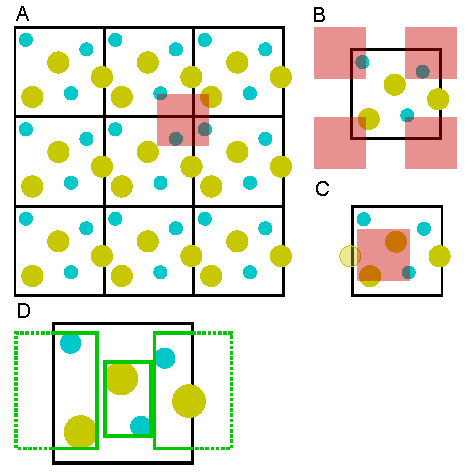
\includegraphics[width=8.0cm, bb=6 3 220 224]{fig1.eps}
    \caption{Methods to handle R-Tree on periodic boundary conditions.
    (\textbf{A})
    By copying the unit cell for each dimension along periodicity, normal R-Tree
    can manage objects that are associated with periodic images.
    (\textbf{B})
    By adding extensional query translated for each periodic images, R-Tree can
    detect objects that are beyond boundary.
    (\textbf{C})
    With the method described in \textbf{B}, finite sized objects could be
    overlooked when queries that is inside of the boundary are not copied.
    (\textbf{D})
    This is the method proposed in this paper. Forming rectangles according to
    the periodicity, R-Tree can organize objects on periodic boundary
    conditions.}
    \label{fig-method-rtree-pbc}
\end{figure}

\section*{Methods}

Here I introduce some operations to modify and handle rectangles on PBCs.
I do not modify the algorithm to grow and maintain an R-Tree at all.
Hence, in this setion, I do not show algorithm to construct R-Tree itself.
It means that this method is potentially applicable for some of the R-Tree
variants and the other spatial indexing methods that is based on BVH and
uses AABBs.

Because the rectangles used in R-Tree are axis-aligned, it is enough to show an
operation for one dimension to provide the whole algorithm.
Applying it to each dimensions successively, these operations can be extended
for higher dimension cases.

\paragraph{Representation of PBCs.}
Here, I consider only cuboids as an unit cell of the PBCs. I assume all the
coordinates of the objects are restricted to be inside of the unit cell.
There are well-known alrogithm to restrict coordinates and vectors to the unit
cell. In this paper, I call them as \textbf{RestrictPosition} and
\textbf{RestrictVector}, respectively.

\paragraph{Representation of AABBs.}
There are three common representations for AABBs
(figure~\ref{fig-rectangle-rep})~\cite{real-time-collision-detection}.
The first one is a pair of the minimum and maximum coordinate values
in each dimension.
The second one is a pair of the minimum coordinate values and its width in each
dimension.
The third one is a pair of the center position and half-width in each dimension.
Here, I call it as min-max, min-widths, and center-radius representation,
respectively.

Because the method proposed in this paper quite often uses center position of
an AABB, here I employ center-radius representation. It makes the processes
simple, but this representation is not indispensable because the center position
can be calculated with another representation.

\begin{eqnarray}
    rectangle = \{center, radius\} \nonumber
\end{eqnarray}

Clearly, since all the representations have identical information about an AABB,
one can convert one representation to another. Algorithm\ref{center_aabb} and
\ref{radius_aabb}, provide ways to convert the min-max representation to
the center-radius representation according to the PBCs.
It should be noted that the maximum coordinate value might be smaller than the
corresponding minimum coordinate value because all the coordinates are
restricted to inside of the unit cell by transposing. It shows that the AABB
sticks out of the boundary.

\begin{figure}[thb]
    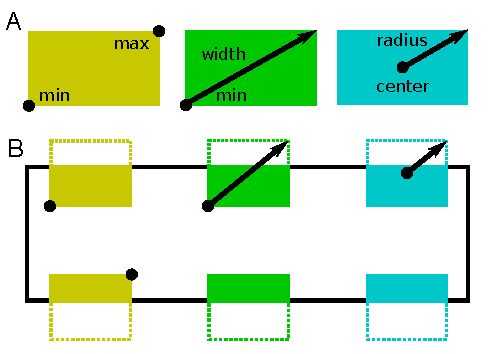
\includegraphics[width=8.0cm, bb=2 6 226 165]{fig-rect-rep.eps}
    \caption{
    (\textbf{A})
    Three popular representations of an AABB. First one is min-max,
    second one is min-widths, and third one is center-radius representation,
    respectively.
    (\textbf{B})
    Three representations on PBCs. The AABBs are colored in the same way as
    \textbf{A}.
    }
    \label{fig-rectangle-rep}
\end{figure}

\begin{algorithm}[htb]
    \caption{calculate the centroid of an AABB on PBCs.}
    \label{center_aabb}
    \begin{algorithmic}
        \State $U \gets$ maximum coordinate values of an AABB
        \State $L \gets$ minimum coordinate values of an AABB
        \State $B \gets$ the unit cell of a boundary
        \Function{CentroidAABB}{$U, L, B$}
            \If{$U < L$}
                \State $C \gets (U + B.width + L) / 2$
            \Else
                \State $C \gets (U + L) / 2$
            \EndIf
            \State \Return $C$
        \EndFunction
     \end{algorithmic}
\end{algorithm}

\begin{algorithm}[htb]
    \caption{calculate the width of an AABB on PBCs.}
    \label{radius_aabb}
    \begin{algorithmic}
        \State $U \gets$ maximum coordinate values of an AABB
        \State $L \gets$ minimum coordinate values of an AABB
        \State $B \gets$ the unit cell of a boundary
        \Function{WidthAABB}{$U, L, B$}
            \If{$U < L$}
                \State $W \gets U + B.width - L$
            \Else
                \State $W \gets U - L$
            \EndIf
            \State \Return $W$
        \EndFunction
     \end{algorithmic}
\end{algorithm}

\paragraph{Expanding AABBs according to PBCs.}
Expanding an AABB to ensure it contains a new contents is one of the most
important operations in an R-Tree algorithms.
Because the total area that is covered by AABBs in the nodes of an R-Tree
affects the efficiency of spatial searching, it is needed to find the way to
make the area of rectangle in each node as small as possible.

The algorithm to find the minimum expansion of AABB to contain another AABB on
PBCs is shown in algorithm ~\ref{expand_aabb_aabb}.
The size of bounding box that contains two rectangles is determined by the
distance between their center points because of the symmetry of a rectangule.
Therefore, by minimizing the distance between their centroids, the minimum
expansion can be found. To minimize the distance between two points on PBCs,
the \textbf{RestrictVector} can be used.

For the case of a point, it become simpler as described in the algorithm
~\ref{expand_aabb_point}. By minimizing the distance between centroid of the
rectangle and the point to be contained, the minimum expansion can be found.

\begin{algorithm}[htb]
    \caption{expand AABB so that it contains another AABB}
    \label{expand_aabb_aabb}
    \begin{algorithmic}
        \State $R1 \gets$ AABB to be expanded
        \State $R2 \gets$ rectangle to be contained
        \State $B  \gets$ boundary
        \Function{ExpandAABB}{$R1, R2, B$}
            \State $dc \gets R2.center - R1.center$
            \State $dc \gets$ \Call{RestrictVector}{dc, B}

            \State $l1 \gets R1.center - R1.radius$
            \State $u1 \gets R1.center + R1.radius$
            \State $l2 \gets (R1.center + dc) - R2.radius$
            \State $u2 \gets (R1.center + dc) + R2.radius$

            \State $L  \gets \Call{min}{l1, l2}$
            \State $U  \gets \Call{max}{u1, u2}$
            \State $C  \gets (L + U) / 2$
            \State $HW \gets (U - L) / 2$
            \State $C  \gets$ \Call{RestrictPosition}{C, B}

            \State \Return $\{C, HW\}$
        \EndFunction
     \end{algorithmic}
\end{algorithm}

\begin{algorithm}[htb]
    \caption{expand AABB so that it contains a point}
    \label{expand_aabb_point}
    \begin{algorithmic}
        \State $R \gets$ AABB to be expanded
        \State $P \gets$ point to be contained
        \State $B \gets$ boundary
        \Function{ExpandAABB}{$R, P, B$}
            \State $dc \gets P - R.center$
            \State $dc \gets$ \Call{RestrictVector}{dc, B}

            \State $l \gets R.center - R.radius$
            \State $u \gets R.center + R.radius$

            \State $L  \gets \Call{min}{l, P}$
            \State $U  \gets \Call{max}{u, P}$
            \State $C  \gets (L + U) / 2$
            \State $HW \gets (U - L) / 2$

            \State $C \gets$ \Call{RestrictPosition}{C, B}
            \State \Return $\{C, HW\}$
        \EndFunction
     \end{algorithmic}
\end{algorithm}



\paragraph{Detecting an object includes or intersects the other object}

To find an object in an R-Tree, the algorithm is needed to check whether an
rectangle intersects or be inside of another rectangle.
It also can be determined by using the minimum distance between centroids of the
rectangles.
The algorithm for the center-radius representation can be applied after
restricting the inter center points vector.

\begin{algorithm}[tbh]
    \caption{Check whether an AABB is inside of an AABB}
    \begin{algorithmic}
        \State $R1 \gets$ rectangle
        \State $R2 \gets$ rectangle that might be inside of R1
        \State $B  \gets$ boundary
        \Function{IsAABBInsideOfAABB}{$R1, R2, B$}
            \State $dc \gets R1.center - R2.center$
            \State $dc \gets$ \Call{RestrictVector}{dc, B}

            \State \Return \Call{abs}{dc} $\leq (R1.radius - R2.radius)$
        \EndFunction
     \end{algorithmic}
\end{algorithm}

\begin{algorithm}[tbh]
    \caption{Check whether a point is inside of an AABB}
    \begin{algorithmic}
        \State $R \gets$ rectangle
        \State $P \gets$ point that might be inside of R
        \State $B \gets$ boundary
        \Function{IsPointInsideOfAABB}{$R, P, B$}
            \State $dc \gets R.center - P$
            \State $dc \gets$ \Call{RestrictVector}{dc, B}
            \State \Return \Call{abs}{dc} $\leq R.radius$
        \EndFunction
     \end{algorithmic}
\end{algorithm}

\begin{algorithm}[tbh]
    \caption{Check whether an AABB intersects to another AABB}
    \begin{algorithmic}
        \State $R1 \gets$ rectangle
        \State $R2 \gets$ rectangle that might intersect to R1
        \State $B  \gets$ boundary
        \Function{IntersectsAABB}{$R1, R2, B$}
            \State $dc \gets R.center - R.center$
            \State $dc \gets$ \Call{RestrictVector}{dc, B}
            \State \Return \Call{abs}{dc} $\leq (R1.radius + R2.radius)$
        \EndFunction
     \end{algorithmic}
\end{algorithm}

\section*{Results}

The codes that are used for this paper is available on GitHub
(\url{http://github.com/ToruNiina/periortree}).

The three steps of expansion of an AABB to contain rectangles is shown in
figure~\ref{fig-result}A.
Here, there is only one bounding box in the figure.
Because it lies beyond the boundary, the periodic image of box is shown separately.

In figure~\ref{fig-result}B the result of a query is shown. It successfully
detects an object that locates beyond the boundaries. It should be noted that
while there are four rectangles drawn in the second panel of figure
~\ref{fig-result}B, actually there is only one rectangle.

\begin{figure}[htb]
    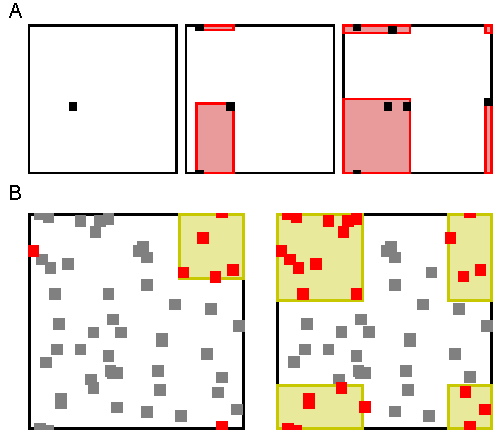
\includegraphics[width=8.4cm, bb=4 6 237 212]{fig-result-expand-intersect.eps}
    \caption{
    (\textbf{A})
    The three steps to expand AABB colored in red to contain black rectangles.
    It can be seen that the AABB are expanded beyond the boundary.
    (\textbf{B})
    The result of querying objects that intersect to yellow rectangle.
    The object contained in the R-Tree is shown as small square boxes.
    The boxes that are detected as intersecting to the query rectangle is
    colored in red.
    }
    \label{fig-result}
\end{figure}

\section*{Conclusion}

In this paper, the novel method for applying PBCs to R-Trees is introduced.
Proposed method is capable of containing not only sizeless points but also
objects with finite size. The method can remove the necessity of both storing
extensional objects and replicating queries. Moreover, it reduces the
size of each node in the natural way on PBCs.

On the other hand, the method introduces tiny but additional costs into each
procedures for maintaining R-Tree and checking geometrical conditions because it
considers the PBCs for all of the steps of searching objects, containing new
objects. It might decrease the efficiency of the R-Tree in some case.

As described before, since the method is only for modifying and handling
rectangles on PBCs, it can essentially be applied for the other R-Tree variants
or the other kind of spatial indexing methods.

Because the adaptation of spatial indexing to a system on PBCs has a chance to
accelerate many kind of sientific simulations, it is expected that this novel
method will have an important role for the simulations that will be performed in
the next decade.

\bibliographystyle{unsrt}
\bibliography{library}{}

\end{document}
